% !TEX encoding = UTF-8 Unicode
 \documentclass[
	12pt,	
	openany,			
	oneside,			
	a4paper,			
	english,			
	french,			
	spanish,			
	brazil,	
	]{abntex2}
 
\usepackage{lmodern}
\usepackage[T1]{fontenc}
\usepackage[utf8]{inputenc}
\usepackage{indentfirst}
\usepackage{color}
\usepackage{graphicx}
\usepackage{microtype}
\usepackage{float}

\usepackage[subentrycounter,seeautonumberlist,nonumberlist=true]{glossaries}

\usepackage[brazilian,hyperpageref]{backref}
\usepackage[alf]{abntex2cite}
 
\titulo{Especificações de Requisitos - Pack The Bag}
\autor{Daniel Yoshizawa e Jacqueline Cardozo}
\local{Florianópolis, SC, Brasil}
\data{14 de Setembro de 2016}
\orientador{Ricardo Pereira e Silva}
\tipotrabalho{Especificações de Requisitos}
\preambulo{Especificações de Requisitos para o jogo Pack the Bag feito para a disciplina de 
Analise e Projeto de Sistemas ministrada pelo professor Ricardo Pereira e Silva}
\definecolor{blue}{RGB}{41,5,195}
 
\makeatletter

\hypersetup{
		pdftitle={\@title}, 
		pdfauthor={\@author},
		pdfsubject={\imprimirpreambulo},
		pdfcreator={LaTeX with abnTeX2},
		pdfkeywords={abnt}{latex}{abntex}{abntex2}{requisitos}{packthebag},
		colorlinks=true,
	    	linkcolor=blue,
    		citecolor=blue,
	    	filecolor=magenta,
		urlcolor=blue,
		bookmarksdepth=4
}
\makeatother

\setlength{\parindent}{1.3cm}
 
\setlength{\parskip}{0.2cm}
 
\makeindex

\begin{document}
 
\frenchspacing
\imprimircapa

\pdfbookmark[0]{\contentsname}{toc}
\tableofcontents*
\cleardoublepage
\textual

\chapter*[Introdução]{Introdução}
\addcontentsline{toc}{chapter}{Introdução}
 
O objetivo do projeto é desenvolver um jogo virtual em rede utilizando a linguagem Java, 
com o intuito de preencher malas com blocos de formas e cores variados de maneira que o máximo desta seja preenchido.

\chapter{Visão Geral}
 
\section{Arquitetura do Programa}
\begin{itemize}
\item Programa orientado a objetos, escrito em Java, utilizando a biblioteca Slick2D;
\item Aplicação distribuída cliente-servidor utilizando o NetGamesNRT;
\end{itemize}

\section{Descrição do Jogo}

Dois jogadores disputam por peças para preencher suas malas, com o objetivo de usar o máximo de peças possíveis para deixar o mínimo de espaços em branco na sua mala. As peças serão agrupadas por cores que possuirão diferentes pontuações. Ao final, quando não houver mais posições disponíveis para peças em ambas as malas, os jogadores serão pontuados. Quem tiver mais pontos ganha.

A complexidade se dá em escolher as peças certas das categorias certas e reduzir a quantidade de peças que o adversário pode utilizar para ganhar mais pontos. Serão utilizadas peças do padrão Tetris e a mala em forma de grade. Também existirão categorias por cores de peças. As peças dentro das categorias com maior pontuação vão aparecer com menor frequência.

A grade terá tamanho variado, quadrados e retangulares. Cada peça pode assumir quatro posições pré-determinadas, o jogador não terá a opção de virar as peças. Estas peças podem assumir qualquer cor das categorias disponíveis. Não serão escolhas randômica, e sim um algoritmo de seleção para controlar a dificuldade.

A cada turno, um grupo novo de 3 peças serão apresentadas e o jogador da vez escolhe uma peça conforme sua estratégia e a arrasta para a posição desejada na grade. Logo após, passando o turno para o adversário o qual repete o processo até que não exista mais posições disponíveis nas malas de ambos os jogadores. Caso um jogador ocupe todas as posições disponíveis antes do outro, o jogador que ainda possuir espaços poderá continuar jogando.
 
\section{Detalhes de Implementação}

O jogo será desenvolvido em cima do framework Slick2D para aproveitar os padrões de projetos comuns a jogos, como o game loop, pools, commands entre outros, assim como a integração com engines de áudio e renderização gráfica.

\section{Fluxo do Jogo}

\subsection{Posição Inicial}

O jogo iniciará quando os dois jogadores estiverem conectados, o algoritmo escolherá um dos jogadores aleatoriamente para começar a jogada. 

\subsection{Jogadas}

O jogador da vez escolherá uma peça dentro do catálogo de peças disponíveis e a posicionará na sua grade. O jogador poderá fazer uso de estratégia ao escolher a peça de uma categoria a fim de obter mais pontos ou dificultar o jogo do adversário. Após posicionar sua peça, o jogador passa a vez para o adversário.

\subsection{Objetivo do Jogo}

O jogo chega ao seu final quando as grades de ambos jogadores não possuir mais espaços para receber peças.

\section{Regras do Jogo}

\begin{itemize}
\item Cada jogador seleciona e adiciona em sua grade apenas uma peça por turno;
\item A peça deve caber e não sobrepor outras peças na grade;
\item O jogador tem o máximo de um minuto para realizar a sua jogada em um turno;
\item O jogador tem autorização para adicionar peças apenas na sua grade;
\item O jogador poderá continuar suas jogadas caso ainda tenha espaço disponível para peças em sua grade e haja peças disponíveis, mesmo que o adversário não tenha mais espaço em sua grade;
\end{itemize}

\section{Premissas de desenvolvimento}

O software deverá :

\begin{itemize}
\item Ser implementado em linguagem de programação Java, utilizando paradigma de orientação a objetos, devendo executar em qualquer plataforma que disponha de máquina virtual Java;
\item Apresentar uma interface gráfica bidimensional (2d);
\item Ser um jogo virtual em rede, na modalidade jogador contra jogador, utilizando o framework NetGamesNRT;
\end{itemize}

\chapter{Requisitos de Software}

\section{Requisitos Funcionais}
\begin{itemize}
\item Conectar - O programa deve apresentar uma opção conectar, para estabelecer conexão com o servidor. O jogador devera definir o nome que o identificará durante a partida nesta etapa;
\item Desconectar - O jogo deve apresentar a opção desconectar, permitindo ao jogador desconectar do servidor, encerrando assim uma possível partida em andamento;
\item Iniciar Partida - O programa deve apresentar uma opção iniciar para que a partida tenha inicio. É necessário que os dois jogadores estejam conectados ao servidor para iniciar uma nova partida;
\item Selecionar peça - As peças devem ser geradas no inicio do turno, podendo ser selecionadas e arrastadas até a posição desejada, está ficara na posição caso não colida com nenhuma peça já colocada na grade ou com os limites da grade;
\item Sair da partida - O programa deve apresentar uma opção sair ao terminar a partida, que fará o programa voltar a tela inicial;
\end{itemize}

\section{Requisitos Não Funcionais}
\begin{itemize}
\item Especificações de projeto - Software escrito na linguagem de programação Java, e especificação feita em UML segunda versão;
\item Interface gráfica para o usuário - O programa deverá ter interface gráfica única, partilhada pelos usuários;
\item Peças - Serão geradas peças no padrão Tetris, podendo assumir diferentes cores;
\item Tecnologia de interface gráfica para usuário - A interface gráfica será desenvolvida a partir da biblioteca Slick2d;
\end{itemize}

\chapter{Esboço da Interface Gráfica}
\begin{figure}[H]
  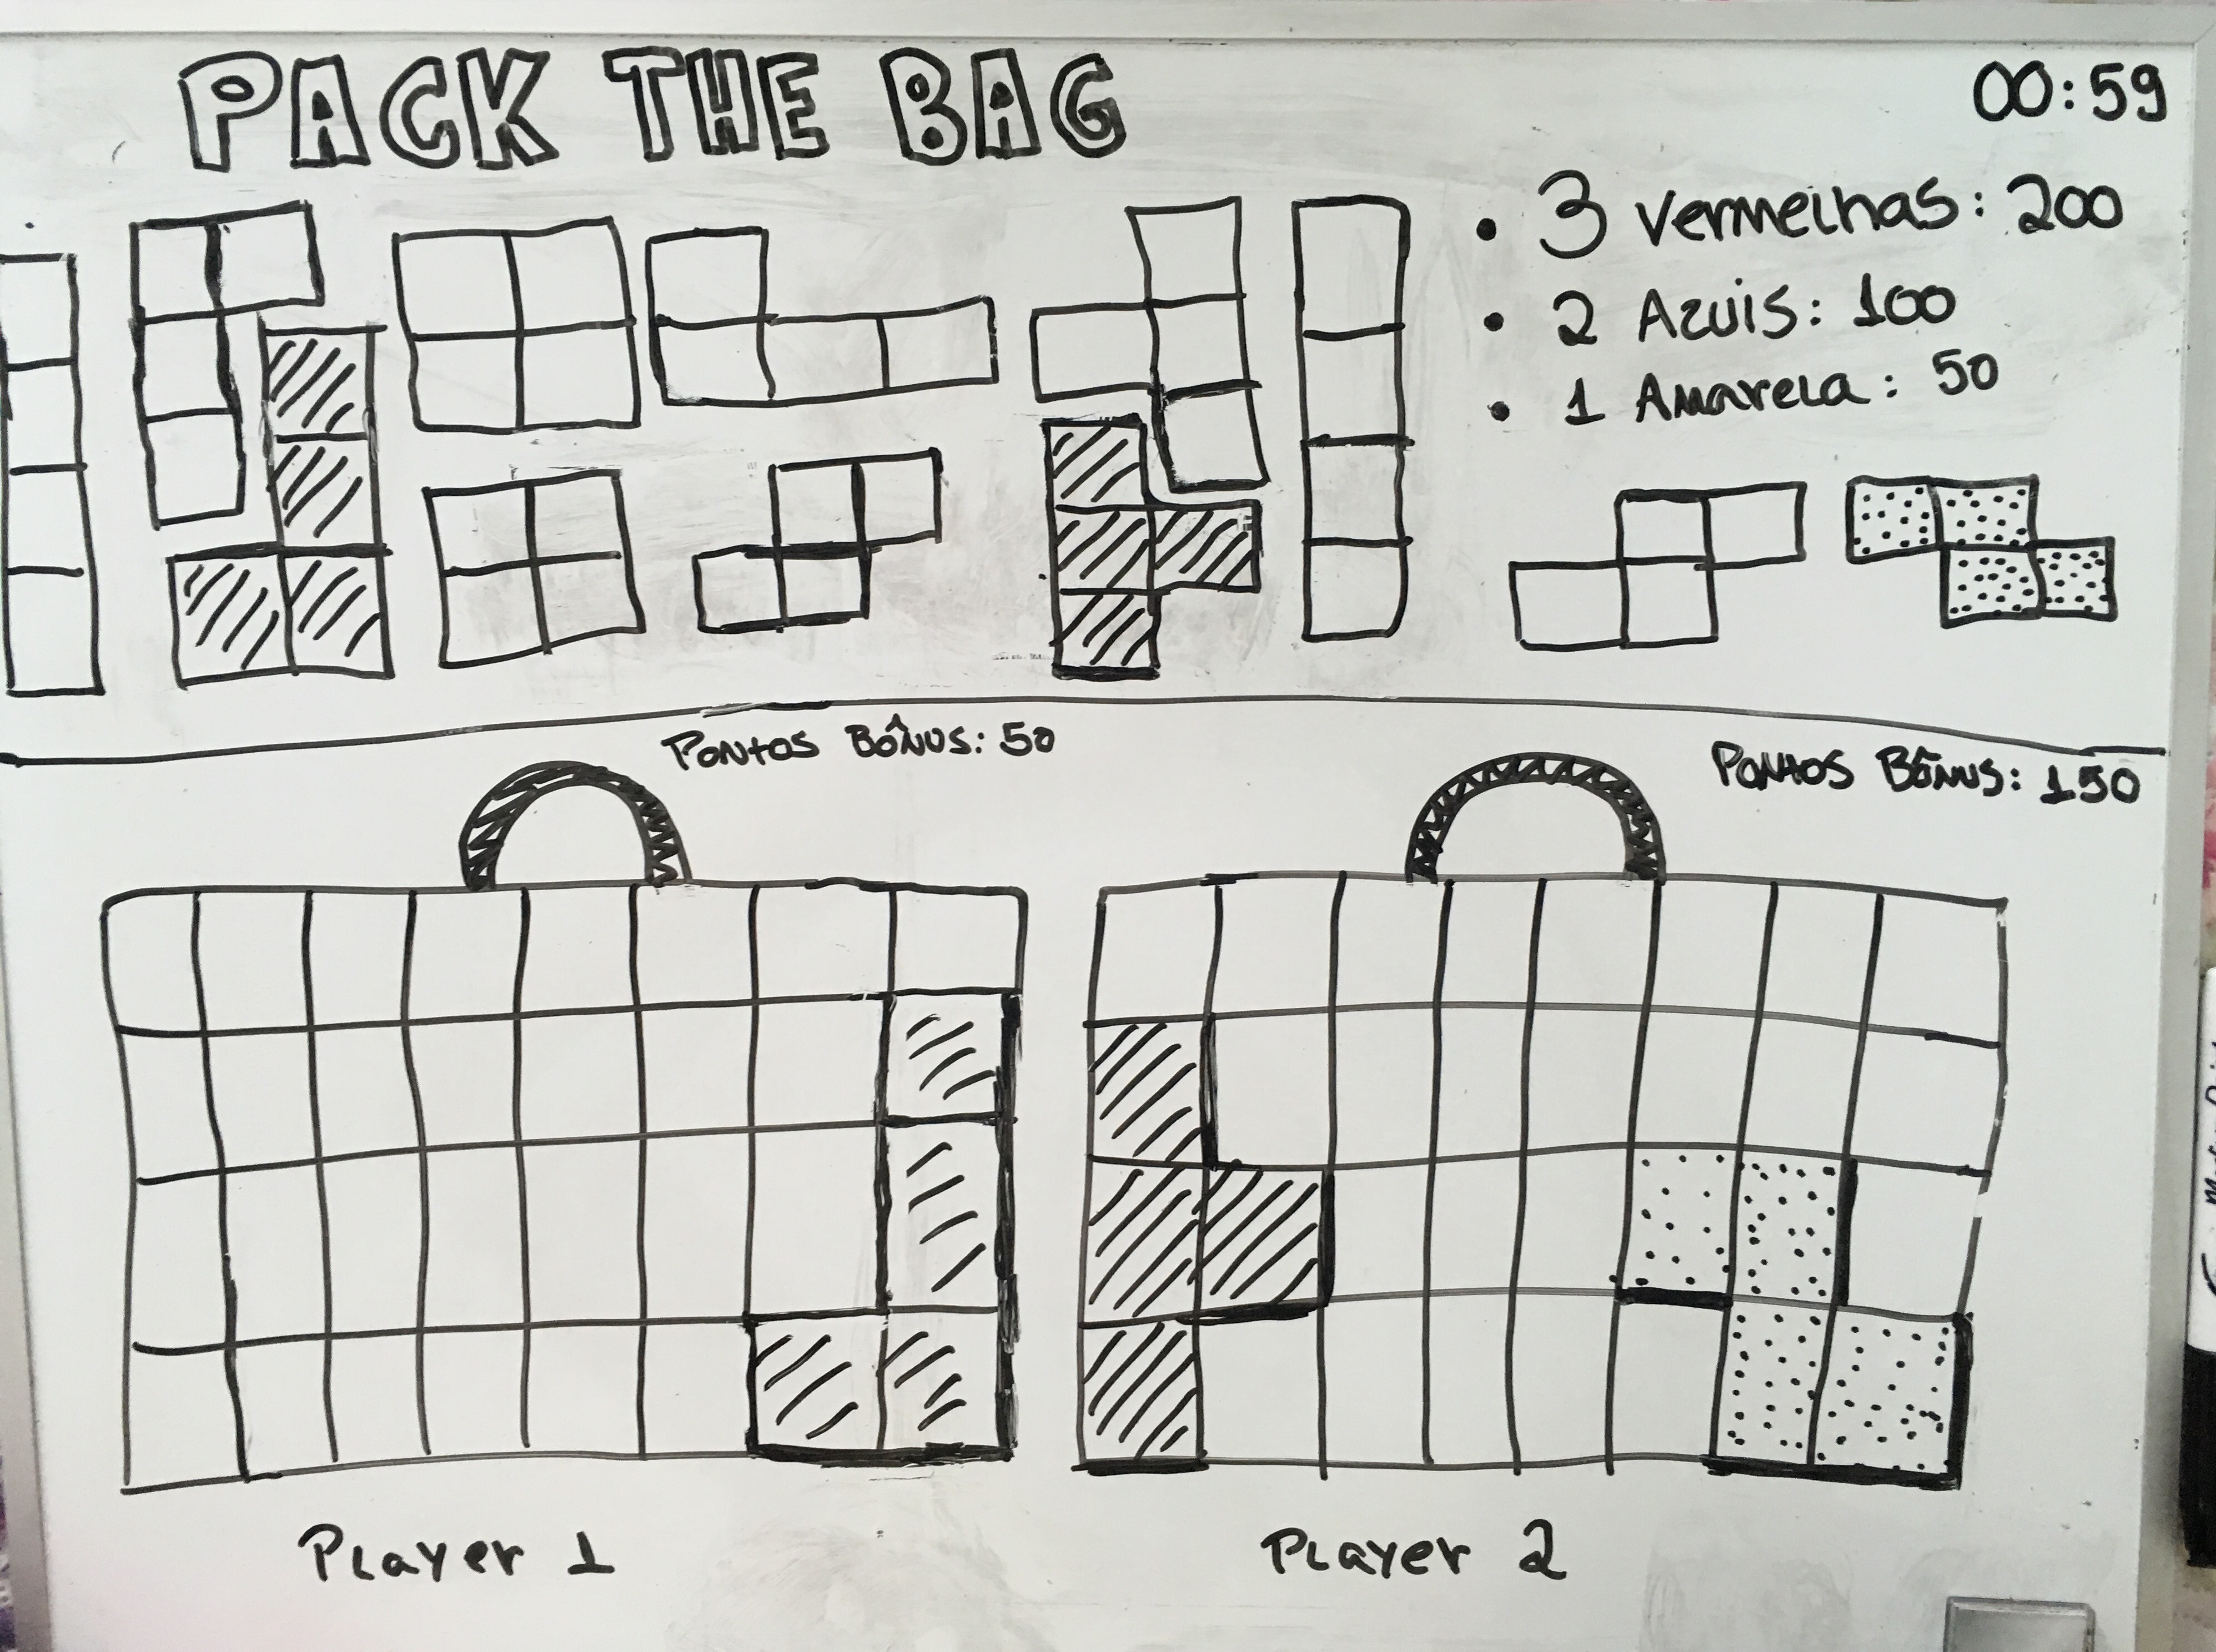
\includegraphics[width=\linewidth]{File_000.jpeg}
  \caption{Esboço da Interface Gráfica}
  \centering
  \label{fig:esboco}
\end{figure}

\include{abntex2-modelo-include-comandos}
 
\end{document}
